\newpage
\section{Data and summary statistics}
\subsection{Household panel}
The data used comes from the Tanzania National Panel survey (NPS) 2008-9, 2010-11 and 2012-13, implemented by the Tanzania National Bureau of Statistics and downloaded from the World Bank LSMS microdata catalogue. The survey covers 3,265 households in 26 districts containing 409 Enumeration Areas (EAs), and is designed to be representative of Tanzania as a whole. Within each EA (village) 8 households were randomly selected. The survey made particular effort to track respondents, with all adult former households members tracked to new location, resulting in over 97\% of the round 1 households being re-interviewed in round 2 and a total panel attrition rate of 4.8\%. The data includes weightings of the probability that an observation was included in the survey to take into account the fact that some areas were over surveyed to reflect the higher variance of the variables of interest (for example in cities). 

 
% Table generated by Excel2LaTeX from sheet 'HH stats'
\begin{table}[htbp]

  \centering
  \caption{HH summary stats by wave} \label{HH sum}
    \begin{tabulary}{1\textwidth}{Lcccccc}
    \toprule
          & \multicolumn{2}{c}{Wave 1}        & \multicolumn{2}{c}{Wave 2} &      \multicolumn{2}{c}{Wave 3}   \\
    \midrule
          & Mean  & SD    & Mean  & SD    & Mean  & SD \\
    Per capita consumption &            743,386  &            725,334  &            862,266  &               782,264  &           1,011,279  &          1,090,465  \\
    Rural & 0.65  & 0.48  & 0.68  & 0.47  & 0.65  & 0.48 \\
    Rainfall shock & 0.18     & 0.38  & 0.09  & 0.29  & 0.20  & 0.40 \\
    Education of head (yrs) & 4.76  & 3.57  & 4.84  & 3.65  & 4.96  & 3.70 \\
    Age of head & 45.53 & 15.05 & 45.85 & 15.53 & 46.71 & 16.04 \\
    Head female & 0.25 & 0.43 & 0.26 & 0.43 & 0.28 & 0.446 \\
    Household size & 5.08  & 2.86  & 5.28  & 3.13  & 5.02  & 3.05 \\
    Mobile money use & 0.00  & 0.00  & 0.13  & 0.33  & 0.38  & 0.49 \\
    Own mobile & 0.45  & 0.50  & 0.62  & 0.48  & 0.71  & 0.45 \\
    \textit{Financial access } &       &       &       &       &       &  \\
    Number of loans & 0.07  & 0.30  & 0.10  & 0.35  & 0.12  & 0.39 \\
    Bank account & .     & .     & 0.20  & 0.40  & 0.20  & 0.40 \\
    ROSCA & 0.04  & 0.20  & 0.05  & 0.22  & 0.04  & 0.19 \\
    Wealth index & -0.80 & 2.99 & 0.14 & 2.84 & -0.89 & 2.56 \\
    \textit{Occupational dummies} &       &       &       &       &       &  \\
     Agriculture/ Livestock" & 0.60  & 0.49  & 0.56  & 0.50  & 0.55  & 0.50 \\
     Fishing & 0.02  & 0.14  & 0.01  & 0.12  & 0.01  & 0.12 \\
     Mining & 0.00  & 0.05  & 0.00  & 0.06  & 0.00  & 0.06 \\
     Tourism & 0.00  & 0.02  & 0.00  & 0.02  & 0.00  & 0.02 \\
     Employed: Government & 0.06  & 0.23  & 0.06  & 0.24  & 0.06  & 0.23 \\
     Parastatal & 0.01  & 0.08  & 0.01  & 0.08  & 0.01  & 0.07 \\
     Private sector & 0.09  & 0.28  & 0.11  & 0.31  & 0.12  & 0.33 \\
     NGO/religious & 0.01  & 0.09  & 0.01  & 0.08  & 0.01  & 0.09 \\
     Self-employed (non-agri) w employees & 0.02  & 0.16  & 0.03  & 0.18  & 0.03  & 0.16 \\
     Self-employed (non-agri) w/o employees & 0.15  & 0.35  & 0.14  & 0.35  & 0.15  & 0.36 \\
     Unpaid family work & 0.01  & 0.05  & 0.01  & 0.11  & 0.01  & 0.11 \\
     
     Job seeker & 0.00  & 0.05  & 0.00  & 0.07  & 0.00  & 0.04 \\
    
     Disabled  & 0.00  & 0.03  & 0.02  & 0.15  & 0.03  & 0.17 \\
     No job & 0.01  & 0.12  & 0.02  & 0.13  & 0.02  & 0.13 \\
    \bottomrule
    \end{tabulary}%
        
  \label{tab:addlabel}%
\end{table}%
 

% Table generated by Excel2LaTeX from sheet 'HH stats'
\begin{table}[htbp]
  
  \centering
  \caption{HH Summary stats by mobile money adoption at wave 3} \label{HH adoption}
    \begin{tabulary}{1 \textwidth}{Lcccccc}
    \toprule
          & \multicolumn{2}{c}{Early adopters}       & \multicolumn{2}{c}{Late adopters} & \multicolumn{2}{c}{Non-Adopters} \\
    \midrule
          &  Mean  &  SD   &  Mean  &  SD   &  Mean  &  SD  \\
   
    Per capita consumption &          1,670,892  &          1,374,892  &          1,498,173  &          1,348,243  &               702,110  &          744,725  \\
    Rural &                     0.30  &                     0.46  &                     0.40  &                     0.49  &                      0.81  &                 0.39  \\
    Rainfall shock &                     0.15  &                     0.36  &                     0.16  &                     0.36  &                      0.22  &                 0.42  \\
    Education of head (yrs) &                     7.57  &                     3.97  &                     6.58  &                     3.68  &                      3.93  &                 3.32  \\
    Age of head &                   44.49  &                   13.56  &                   43.62  &                   14.82  &                   48.62  &              16.50  \\
    Head female & 0.22 & 0.41 & 0.25 & 0.43 & 0.29 & 0.45 \\
    Household size &                     4.94  &                     2.74  &                     4.79  &                     3.01  &                      5.16  &                 3.06  \\
    Household wealth index &                     2.23  &                     3.07  &                     1.24  &                     3.04  & -                   0.94  &                 1.74  \\
    Mobile money use &                     0.88  &                     0.33  &                     1.00  &                          -    &                          -    &                     -    \\
    Own mobile &                     0.97  &                     0.18  &                     0.98  &                     0.15  &                      0.54  &                 0.50  \\
    \textit{Financial access } &       &       &       &       &       &  \\
    Number of loans &                     0.26  &                     0.52  &                     0.21  &                     0.50  &                      0.07  &                 0.28  \\
    Bank account &                     0.52  &                     0.50  &                     0.40  &                     0.49  &                      0.07  &                 0.26  \\
    ROSCA &                     0.09  &                     0.29  &                     0.07  &                     0.26  &                      0.02  &                 0.13  \\
    Wealth index & 2.32 & 3.65 & 1.33 & 3.31 & -0.81 & 2.00 \\
    \textit{Occupational dummies} &       &       &       &       &       &  \\
     Agri/ Livestock &                     0.28  &                     0.45  &                     0.34  &                     0.47  &                      0.68  &                 0.47  \\
     Fishing &                          -    &                          -    &                     0.01  &                     0.09  &                      0.02  &                 0.13  \\
     Mining &                     0.00  &                     0.05  &                     0.00  &                     0.07  &                      0.00  &                 0.05  \\
     Tourism &                          -    &                          -    &                          -    &                          -    &                      0.00  &                 0.02  \\
     Employed: Gov &                     0.13  &                     0.34  &                     0.10  &                     0.30  &                      0.03  &                 0.16  \\
     Parastatal &                     0.02  &                     0.15  &                     0.01  &                     0.09  &                      0.00  &                 0.05  \\
     Private sector &                     0.18  &                     0.38  &                     0.19  &                     0.39  &                      0.08  &                 0.27  \\
     NGO/religious &                     0.02  &                     0.13  &                     0.01  &                     0.12  &                      0.00  &                 0.05  \\
     Self-employed (non-agri) with employees &                     0.07  &                     0.26  &                     0.05  &                     0.22  &                      0.01  &                 0.10  \\
     Self-employed (non-agri) w/o employees &                     0.23  &                     0.42  &                     0.22  &                     0.41  &                      0.11  &                 0.32  \\
     Unpaid family work &                     0.01  &                     0.10  &                     0.01  &                     0.11  &                      0.01  &                 0.11  \\
    Job seeker &                          -    &                          -    &                     0.00  &                     0.04  &                      0.00  &                 0.04  \\
     
     Disabled  &                     0.02  &                     0.13  &                     0.02  &                     0.15  &                      0.03  &                 0.18  \\
     No job &                     0.03  &                     0.17  &                     0.02  &                     0.14  &                      0.02  &                 0.13  \\
    \bottomrule
    \end{tabulary}%
    \label{tab:addlabel}%

\end{table}%


The survey included questions on consumption, assets, finance, shocks, household characteristics and village characteristics, as well as detailed agricultural and fisheries information. I combined the data by household since mobile money use is recorded at the household level. Looking at the characteristics of the household head in table \ref{HH sum}, the average household has 5 people, average years of education of the household head is just under 5 years, increasing slightly during the survey. 60\% of household heads worked in agriculture, 10\% in the private sector as paid worker and 15\% were self employed. In 2008-11 annual real per person consumption was 742,386 TZ Shillings (\$450), rising to 802,256 shilling (\$490) in 2010-11 and 1,011,279 (\$568) in 2012-13. 

I generated a wealth index of assets using principal component analysis (PCA). Different components of wealth, such as the number of chickens owned or bicycle ownership, cannot easily be added up. PCA determines the relative importance of variables when seeking to summarize a set of variables. It reduces the set of variables by comparing how similar they are to each other, and based on this creates a new variable called the principal component. The first principal component accounts for the largest variance across the variables. In a wealth index, the first principal component is assumed to represent relative wealth. Based on this, each factor is given a factor weight representing its relative importance in constructing the principal component. I generated a wealth index score based on these factor weights. 

Looking at mobile phone ownership and mobile money use,  in 2008-9, 45\% of households owned at least one mobile phone, increasing to 62\% in 2010-11 and 71\% in 2012-13. 13\% of households had used a mobile money service in 2010-11 and 38\% had by 2012-13. I am interested in both users and non users in villages with mobile money and non-users in villages without mobile money. Therefore I break down the number of villages and households by these categories in Figure \ref{fig:users chart}. This figure shows the large increase in both villages with mobile money agents and mobile money users within these villages. By the second round of the survey 17\% of the communities had a mobile money agent present within the village, and a further 21\% had mobile agents within 5km of the community. By 2012-13, 52\% of the communities had a mobile money agent and a further 13\% were within 5k of one.  
\begin{figure}
\centering
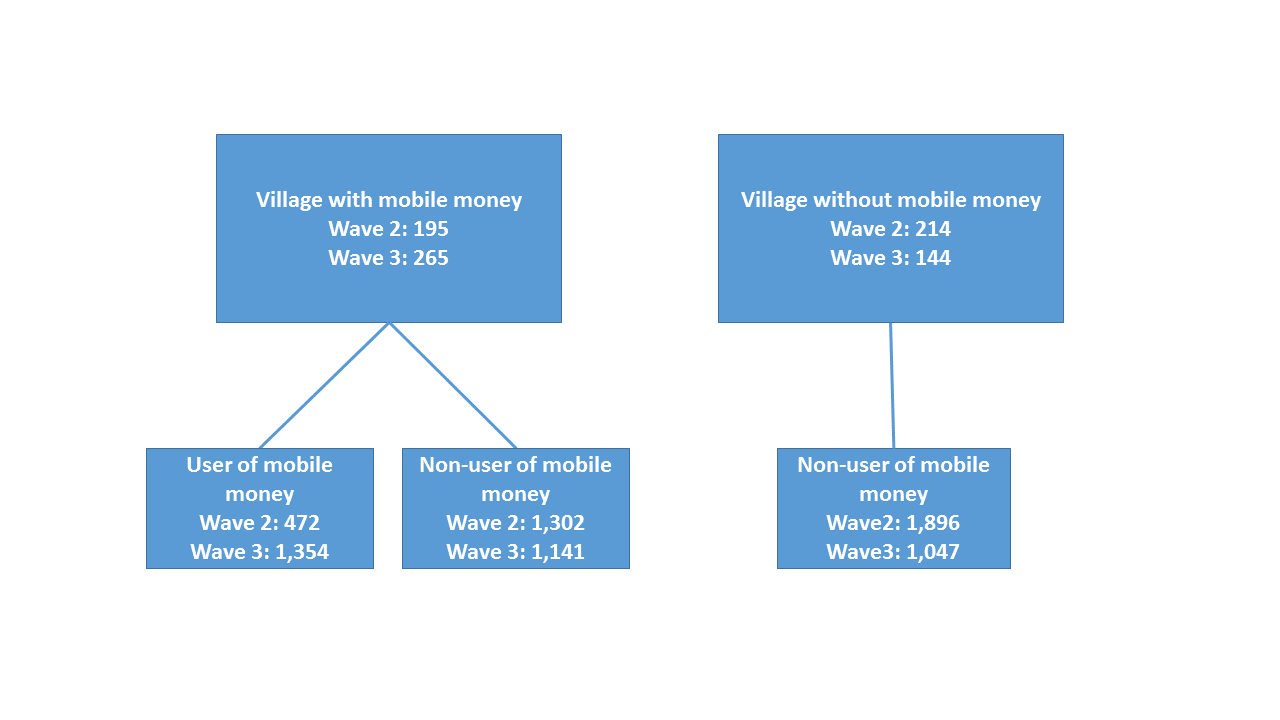
\includegraphics[width=\textwidth,trim= 0 3cm 0 3cm, clip=true, keepaspectratio]{users_chart_} 
\caption{Break down of villages and households by mobile money use} \label{fig:users chart}
\end{figure}

I also examine characteristics by adoption date of mobile money in Table \ref{HH adoption}. Early adopters used mobile money in the second round, 2010-11, and late adopters in the third round, 2012-13. A few people used mobile money in the second round but not in the third. Those who used mobile money are more educated, richer, more likely to live in an urban area and have a bank account and loans, almost always have a mobile phone and are slightly younger than those who don't use mobile money. They are less likely to work in agriculture and more likely to work in the private sector or be self employed. These differences are important to take into account when estimating the impact of mobile money use. 

Sending and receiving money are by far the most popular uses of mobile money, with 67\% of users saying they send money and 82\% of users saying they receive money. These two uses are also given as the most important use of mobile money services by 80\% of respondents. 40\% of people report using mobile money services to save up for emergencies or expenses and 12\% have used it to pay for a good or service. 40\% of people use the service at least monthly. The most common reasons for not using mobile money are no mobile phone, don't understand the service and lack of access to agent, with each of these given in just over a third of responses.  

In the third round of the survey there was detailed data on who sent the remittances to whom using what channel, where from and what their relationship was to the sender. 55\% of remittances were sent via friends and family and 50\% by mobile money. Only 3\% was sent using a bank account, 1\% using Weston Union and 0.4\% using the Post Office. In the past it's likely that the majority of remittances were sent via friends and family with very little sent using any more formal channels. 40\% of remittances were sent by a son or daughter with only 3.5\% sent via a spouse, 7\% by a parent and 17\% by a sibling. 30\% of remittances are sent from Dar Es Salaam. This is consistent with a pattern of a family member migrating to another location such as the city and then sending remittances back to their family. 


\subsection{Rainfall measure}
The panel data contains information on self reported shocks, including whether a household has experienced a drought or flood. This is a dummy equal to one if the household reported that they experienced a drought or flood in the year proceeding the survey wave. To the extent that households misreport or subjectively interpret a rainfall shock, for example saying they experienced a rainfall shock to justify a poor crop yield or exaggerating the importance of a rainfall shock in a year when they have no other shocks, this measure of rainfall shocks will be subject to bias and measurement error. I therefore also calculate a rainfall shock measure per village using data from the NOAA's climate prediction centre FEWS (Famine Early Warning System). This is available at 0.1 degree resolution by latitude and longitude across Africa and was included in the Tanzania NPS summarized at the EA level. 

I define a rainfall shock as more than a 1 standard deviation in absolute values from the 40 year mean by the nearest rainfall station to the village, as used in \cite{jensen2000}.  Deviations from the historic mean capture the extent that rainfall is different from what is expected, and 1 standard deviation is a large difference from normal (on average 200mm difference from an average annual rainfall of 800mm across the entire country). The absolute value is used because either too much or two little rainfall can be harmful. Only deviations greater than 1 standard deviation in absolute value are examined since a little bit too much or too little rain is unlikely to have a big effect, and initially more rain can have a positive effect on crop yields \cite{paxson1992using}. I am only interested in extreme, abnormal, rainfall deviations which could be classified as a drought or flood. The rainfall deviations in millimetres by year are shown in figures \ref{rain09} to \ref{rain12}.    

The mechanism through which rainfall shocks negatively affect income can be varied as I look at both rural and urban households. In rural households, droughts and floods will destroy crops leading to loss of income. In urban areas, flooding is likely to be the main mechanism though which rainfall shocks affect income by preventing people from working and by destroying property. For example, in Dar es Salaam in December 2011 there were severe floods resulting in over 6,000 people being displaced and left homeless. I examine the size of these different mechanisms by examining separately droughts and floods for both urban and rural households. In both these examples remittances can be sent to alleviate the loss of consumption, from urban to rural households after crop destruction and from rural to urban households in the case of severe floods. 

\begin{figure}[h]
\caption{Deviations from mean rainfall, mm}
\centering
\begin{subfigure}[h]{0.45\textwidth}
\caption{July 2009-10}
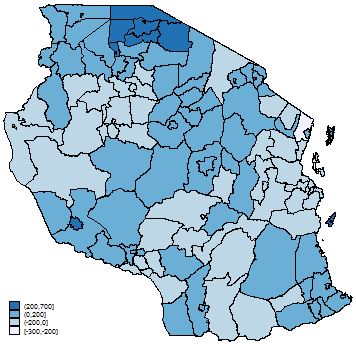
\includegraphics[width=\textwidth,trim= 0cm 0cm 0cm 0cm, clip=true, keepaspectratio]{09_dev_district} \label{rain09}
\end{subfigure}
\begin{subfigure}[h]{0.45\textwidth}
\caption{July 2010-11}
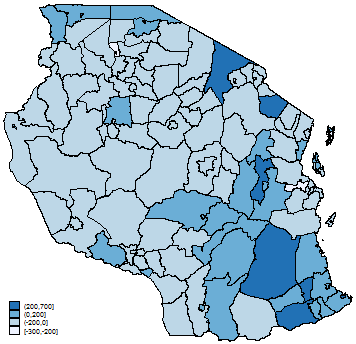
\includegraphics[width=\textwidth,trim= 0cm 0cm 0cm 0cm, clip=true, keepaspectratio]{10_dev_district} \label{rain10}
\end{subfigure}
\begin{subfigure}[h]{0.45\textwidth}
\caption{July 2011-12}
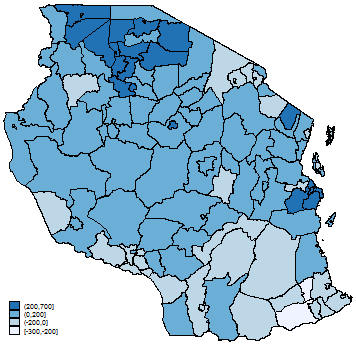
\includegraphics[width=\textwidth,trim= 0cm 0cm 0cm 0cm, clip=true, keepaspectratio]{11_dev_district} \label{rain11}
\end{subfigure}
\begin{subfigure}[h]{0.45\textwidth}
\caption{July 2012-13}
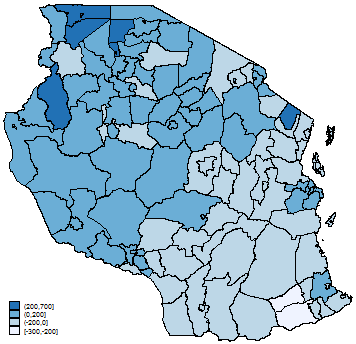
\includegraphics[width=\textwidth,trim= 0cm 0cm 0cm 0cm, clip=true, keepaspectratio]{12_dev_district} \label{rain12}
\end{subfigure}
\end{figure}
\clearpage